\section{Basic Methods}
\label{BasicM}
In order to get some basic understanding of the methods commonly used for iris classification the work presented in an article is implemented. The work implemented is the work of \cite{Khan2017a} described in \textit{Iris Recognition using Machine Learning from Smartphones Captured Images in Visible Light}. In the work the database Warsaw-BioBase containing \gls{vl} images of the iris obtained by smartphones are processed and used to train different classifiers. The images of this database comply with the requirements set for this work mentioned in \autoref{ch:req}. The processing consists of a sequence of steps. The steps included are

\begin{itemize}
\item Iris Location
\item Eyelid Suppression
\item Iris Normalisation
\item Noise Removal
\item Histogram Equalisation 
\item Feature Extraction
\item Training and Classification
\end{itemize}
\autoref{fig:ExWars} shows an example of an image from the database. Before the first step some simple preprocessing is done. The red channel is preserved and the other two colour channels are neglected. This is done because this simulates the use of \gls{nir} light. The result is a greyscale image based on the red channel. In the following sections the implementation of each of the steps is elaborated. 

\begin{figure}[h]
\centering
\begin{subfigure}{.47\textwidth}
\centering
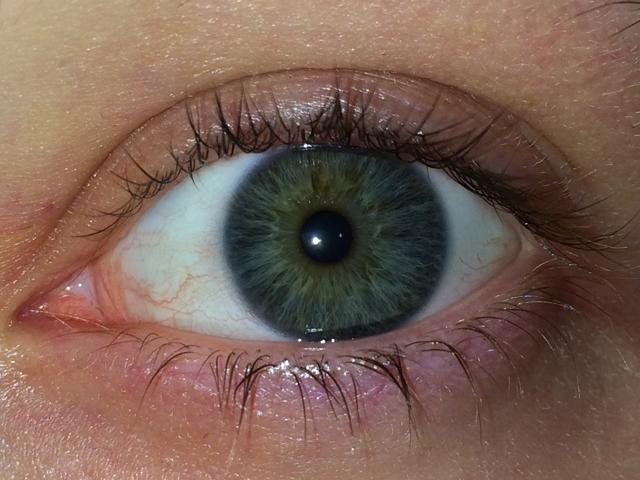
\includegraphics[width=0.90\textwidth]{IMG_1838.jpg}
\caption{Example of visible light image of an iris from the used database.}
\label{fig:ExWars}
\end{subfigure}
~
\begin{subfigure}{.47\textwidth}
\centering
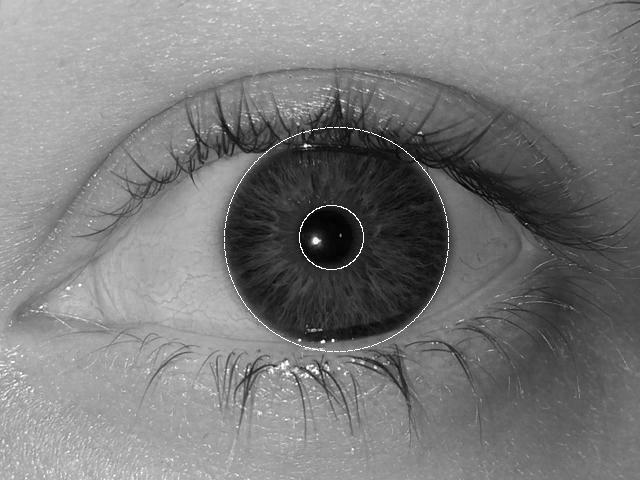
\includegraphics[width=0.90\textwidth]{0002left_13-marked.jpg}
\caption{The eye marked with the identified edges of the iris.}
\label{fig:MarkedI}
\end{subfigure}

\begin{subfigure}{.47\textwidth}
\centering
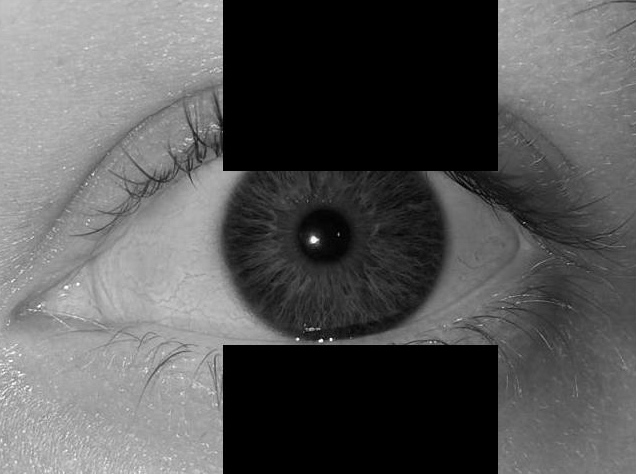
\includegraphics[width=0.9\textwidth]{Eyelid_002_l_13_2.jpg}
\caption{The eye with the eyelid suppression applied.}
\label{fig:IrisSup}
\end{subfigure}
\caption{The original image before and after different steps of processing.}
\end{figure}



\subsection{Iris Extraction}
The first step of processing is locating the iris. For this purpose Daugman's Integro-differential operator is used. The operator identifies the circular contour, which has the greatest change in intensity by varying the three parameters defining the circle $(r,x_0,y_0)$, radius and centre coordinates. The operator is defined by the formula in \autoref{eq:integro_diff}.

\begin{equation}\label{eq:integro_diff}
	\max(r,x_{0},y_{0}){\left|G_{\sigma}{(r)*}{\partial\over \partial_{r}}{\oint_{r,x_{0},y_{0}}}{{I(x,y)\over 2\pi r}dS}\right|}
\end{equation}
Where $I(x,y)$ is the intensity or grey level of the image at the coordinates (x,y), $S$ is the circle, and $G_{\sigma}{(r)}$ is a Gaussian smoothing function.
The method is also used to find the edge between the pupil and the iris. The two identified edges are marked on the input image. \autoref{fig:MarkedI} shows an example of the identified edges of the iris. 

\subsection{Eyelid Suppression}
The annulus, which lies between the two borders identified during the iris extraction might not only contain the iris. The subject might in some cases not open the eyelids fully or the angle of the camera might be such that parts of the iris is covered by the eyelids. Therefore, an algorithm which eliminates the eyelids is used. 
The algorithm is applied on the image cutout of the original image, which is bound by the boundary box of the identified iris. The small image is divided into an upper and a lower part, which are searched for the upper and the lower eyelid respectively. The search is done by using a method with some similarities to Daugman's Integro-differential operator shown in \autoref{eq:integro_diff}, however it applies radon transform. Through the output of the radon transform the lines marking the two eyelids are found and the pixels above or below the two lines respectively are eliminated. The resulting image is shown in \autoref{fig:IrisSup}.

\subsection{Iris Normalisation}
\label{sec:irisnorm}
For the normalisation, Daugman's Rubber Sheet Model is used. The purpose is to get a rectangular image of the iris, which corresponds to taking the annulus covered by the iris region, cutting it open and unfolding or stretching it to a rectangular shape. 

\begin{figure}[h]
\centering
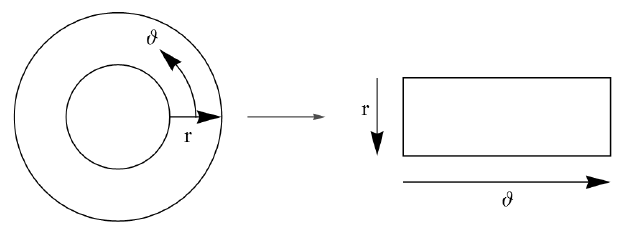
\includegraphics[width=0.8\textwidth]{Daugmans-Rubber-Sheet-Model.png}
\caption{Daugman's Rubber Sheet Model. \citep{Misztal2012}}
\label{fig:DaugSheet}
\end{figure}

The model does this by mapping the iris from the original image to a rectangular image. The mapping is done based on polar coordinates, radius, and angle, $(r,\vartheta)$, where $r\in[0,1]$ and $\vartheta\in[0,2\pi]$. In the rectangular image angle $\vartheta$ is on the x-axis and the radius $r$ is on the y-axis of the image. \autoref{fig:DaugSheet} shows the mapping of the method. This was implemented using a function in the library crated by Libor Masek \citep{LiborMasek2003}. The resolution of the resulting image is dependent on arguments. In this work the dimensions are set to be $64\times512$. The image of the normalised iris is shown in \autoref{fig:SimPolar}. 

\begin{figure}[h]
\centering
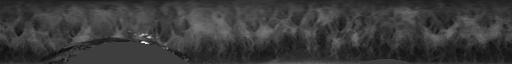
\includegraphics[width=\textwidth]{002polar.jpg}
\caption{The normalised image of the iris before applying functions.}
\label{fig:SimPolar}
\end{figure}

\subsection{Noise Removal}
Though the article uses several well known methods, which are commonly used in processing of images of irises, the descriptions of the methods are quite inadequate. The description of the noise removal is an example hereof. After obtaining the normalised iris, the next step applied is noise removal. The purpose of the noise remover function is to remove noise occurring in the form of eyelashes covering parts of the iris. Usually the pixels showing the lashes will be among the darkest pixels. Since every image of an iris is different and how dark the iris is also varies, a threshold has to be identified adaptively. The article does not describe in depth how this is implemented, it simply states that some histogram analysis is done in order to obtain the lowest pixel values. \autoref{fig:histBif} shows the histogram of the normalised image before any noise removal. 

\begin{figure}[h]
	\centering
	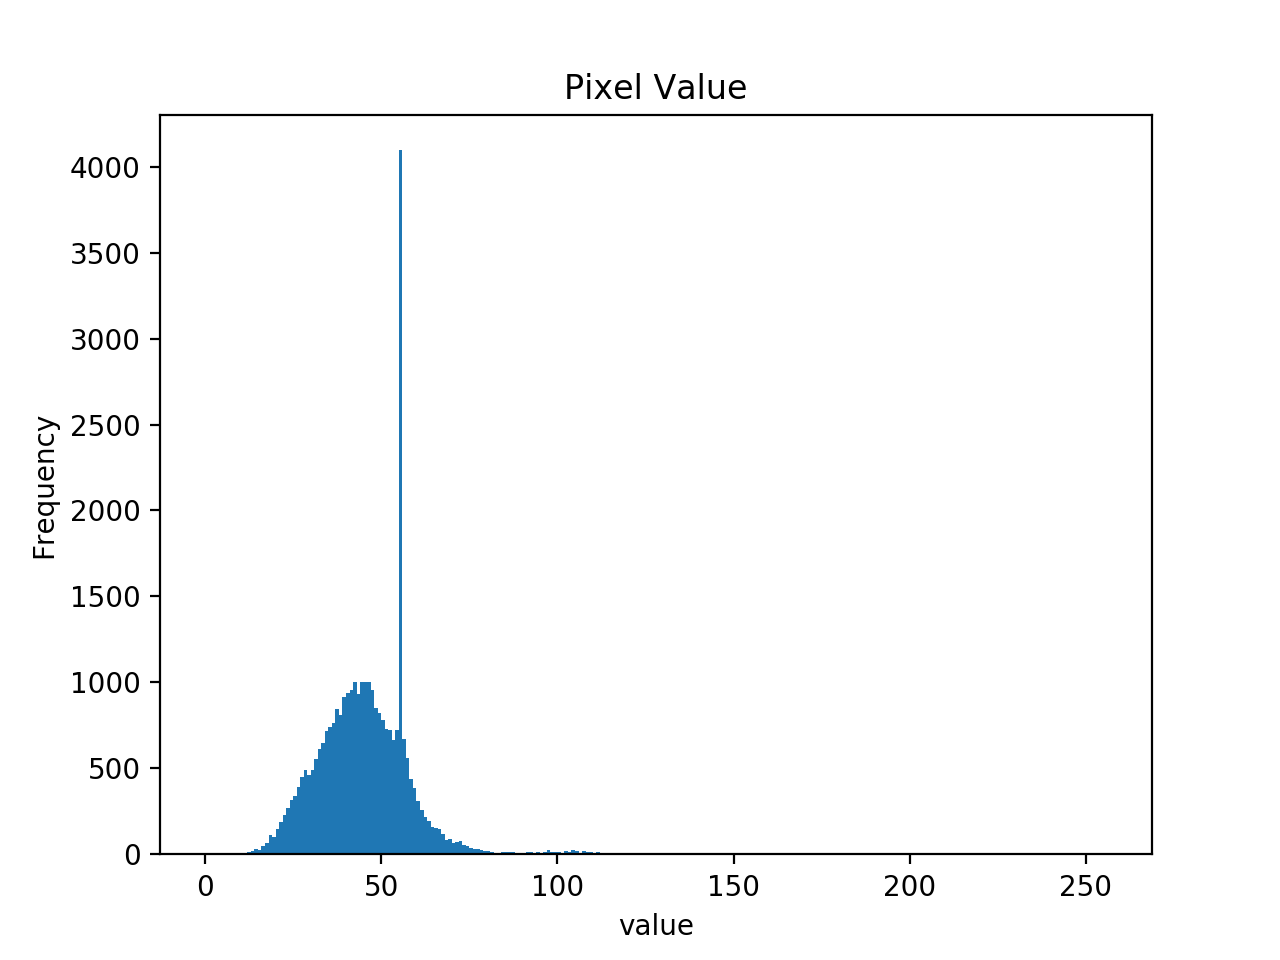
\includegraphics[width=0.7\textwidth]{hist_before.png}
	\caption{The histogram before applying the functions.}
	\label{fig:histBif}
\end{figure}

As the information about the exact approach used in the article is inadequate, an adaptive algorithm is created. The algorithm implemented identifies a threshold value based on the histogram. This is done by first identifying the highest and lowest bin-value, which has a frequency of more than a specified "recognition value", which is set to 10 in this project. The recognition value is introduced to make sure outliers are not defining for the threshold. Afterwards the threshold is calculated by the formula in \autoref{eq:pix_threshold}, where \textit{Fraction} is a parameter set manually defining how large a part of the identified pixel value range has to be thresholded. During the processing in this project \textit{Fraction} is set to be equal to $0.1$. 

\begin{equation}\label{eq:pix_threshold}
	\text{Threshold}=\text{Low~Value}+\text{Fraction}\cdot(\text{High~Value}-\text{Low~Value})
\end{equation}


After the threshold has been found it is applied to all pixels in the image. The pixels lower than the threshold are eliminated and have to be reconstructed from neighbouring pixels. Also here the article provides very limited information about the algorithm applied for reconstruction. Therefore an algorithm was implemented, which restores pixels from non-occluded neighbour pixels. A part of the algorithm identifies the pixels with values lower than the threshold and saves the pixel coordinates of these pixels. The saved pixels are  reconstructed iteratively from neighbouring pixels following the 4-connectivity principle. The pixels are reconstructed when there are at least 2 neighbour pixels they can be reconstructed from. They are only reconstructed from pixels above the threshold, this can be pixels that initially were above the threshold, or it can be pixels that have already been reconstructed. The pixels are reconstructed by assigning the average of the neighbours with values above the threshold as the new pixel value. Once all thresholded pixels have been reconstructed the resulting image is returned.

Because the eliminated pixels are reconstructed only from pixels with a value higher than the threshold there are certain traits that can be expected in the histogram of the reconstructed image. One of the traits is that there is a flatline from 0 to the threshold value. A second trait is that a peak close to the threshold is likely to occur because the eliminated values are reconstructed from neighbours, which are likely to be close to the value of the eliminated pixels. However, the plotted histogram after reconstruction is as shown in \autoref{fig:histSpill}.

\begin{figure}[h]
	\centering
	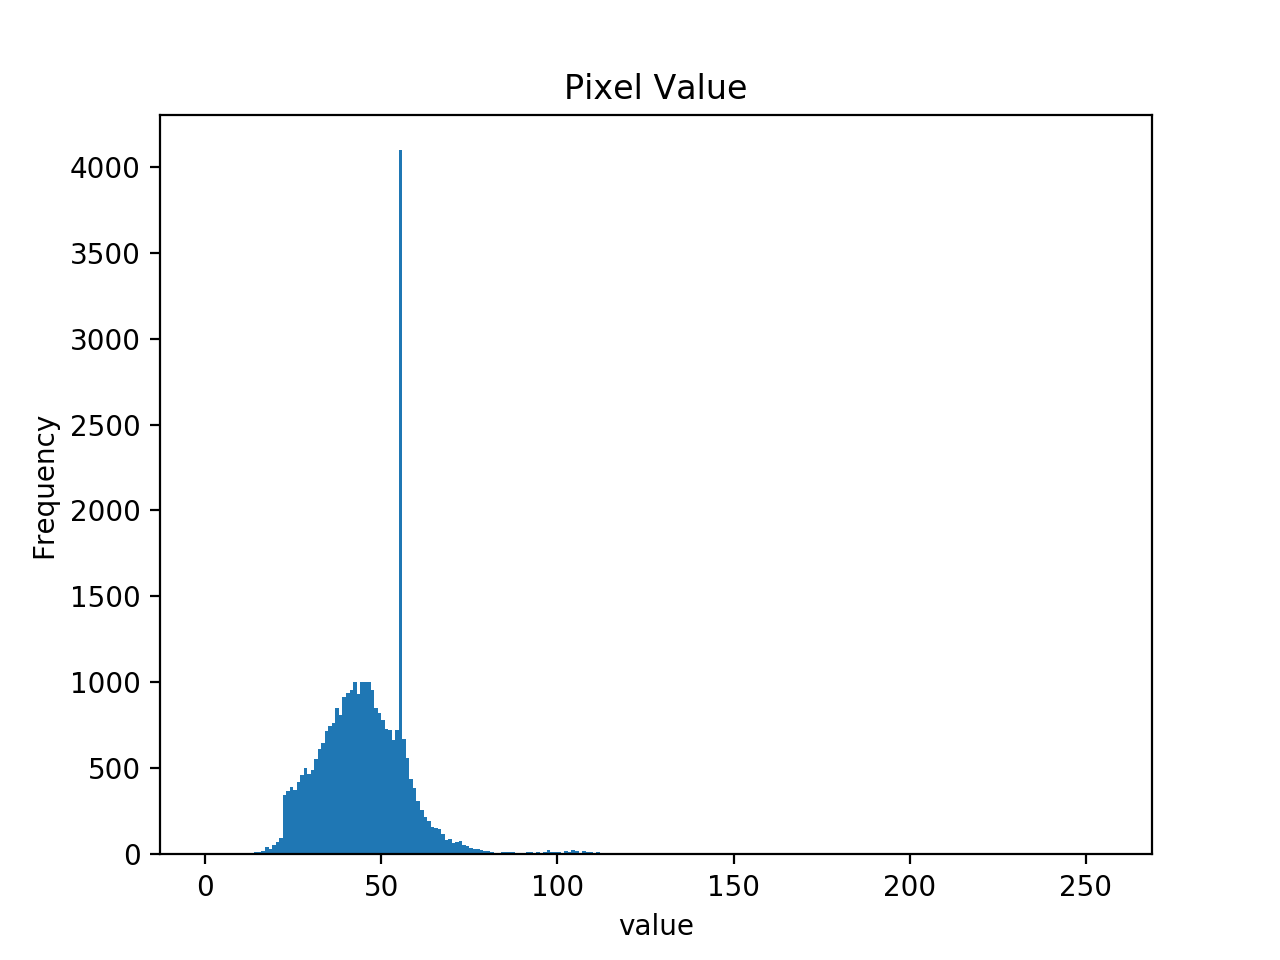
\includegraphics[width=0.7\textwidth]{hist_spill.png}
	\caption{The histogram of the image after reconstruction of pixels.}
	\label{fig:histSpill}
\end{figure}

As can be seen there is a small peak as expected, however, there seem to be a "spill over" across the threshold to the lower values. By closer examination of the code it was discovered that this was caused due to a programming mistake. The mistake was that the values used for reconstruction were obtained from the original image and not from the reconstructed image. Once this mistake was corrected the histogram was as expected as shown in \autoref{fig:histFine}. 

\begin{figure}[h]
	\centering
	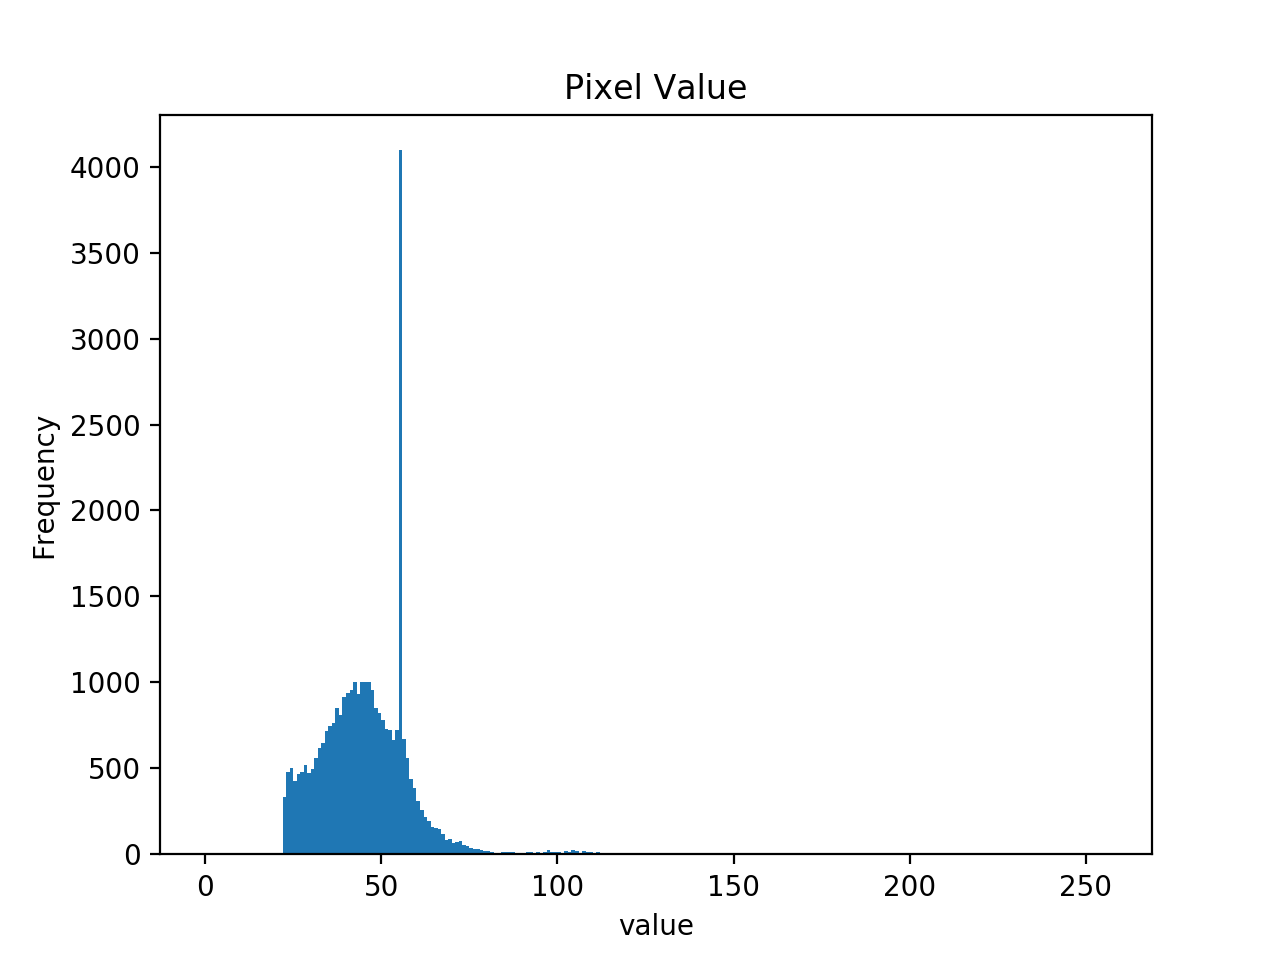
\includegraphics[width=0.7\textwidth]{hist_nicespacing.png}
	\caption{The histogram of the image after applying the corrected noise remover function.}
	\label{fig:histFine}
\end{figure}

In relation to the reconstruction of pixels it should be noted that it could have been done with 8-connectivity, and the iterative process could be split up to more steps, such that pixels are always constructed from as many neighbours as possible. This may give a better reconstruction, however, this has not been investigated. 
Furthermore, small tests showed that the adaptive threshold is difficult to define in an optimal way. If the threshold is too low the eyelash might be reconstructed from edge pixels of the eyelash creating just a lighter eyelash, which is still darker than the iris in the background. If the threshold is higher, it might eliminate the eyelashes, but also be destructive to darker parts of the iris. Maybe this could also be solved if the reconstruction happened based on the neighbourhood and not just the most adjacent neighbour pixels.
 
During implementation the histograms were frequently inspected in order to ensure the results were as expected. \autoref{fig:HistEli} shows a histogram with some eliminated pixel values. It turns out that the function used for generating histograms in python by default takes the range of the pixel values and splits that into as many bins as specified. As a result some of the bins cover a range of values that is entirely between two integer values and thus do not count any instances of pixel values as they are always integers between 0 and 225. This was solved by passing a specific range $[0,256]$ as an argument and then the histogram was as displayed in \autoref{fig:histFine}.

\begin{figure}[h]
	\centering
	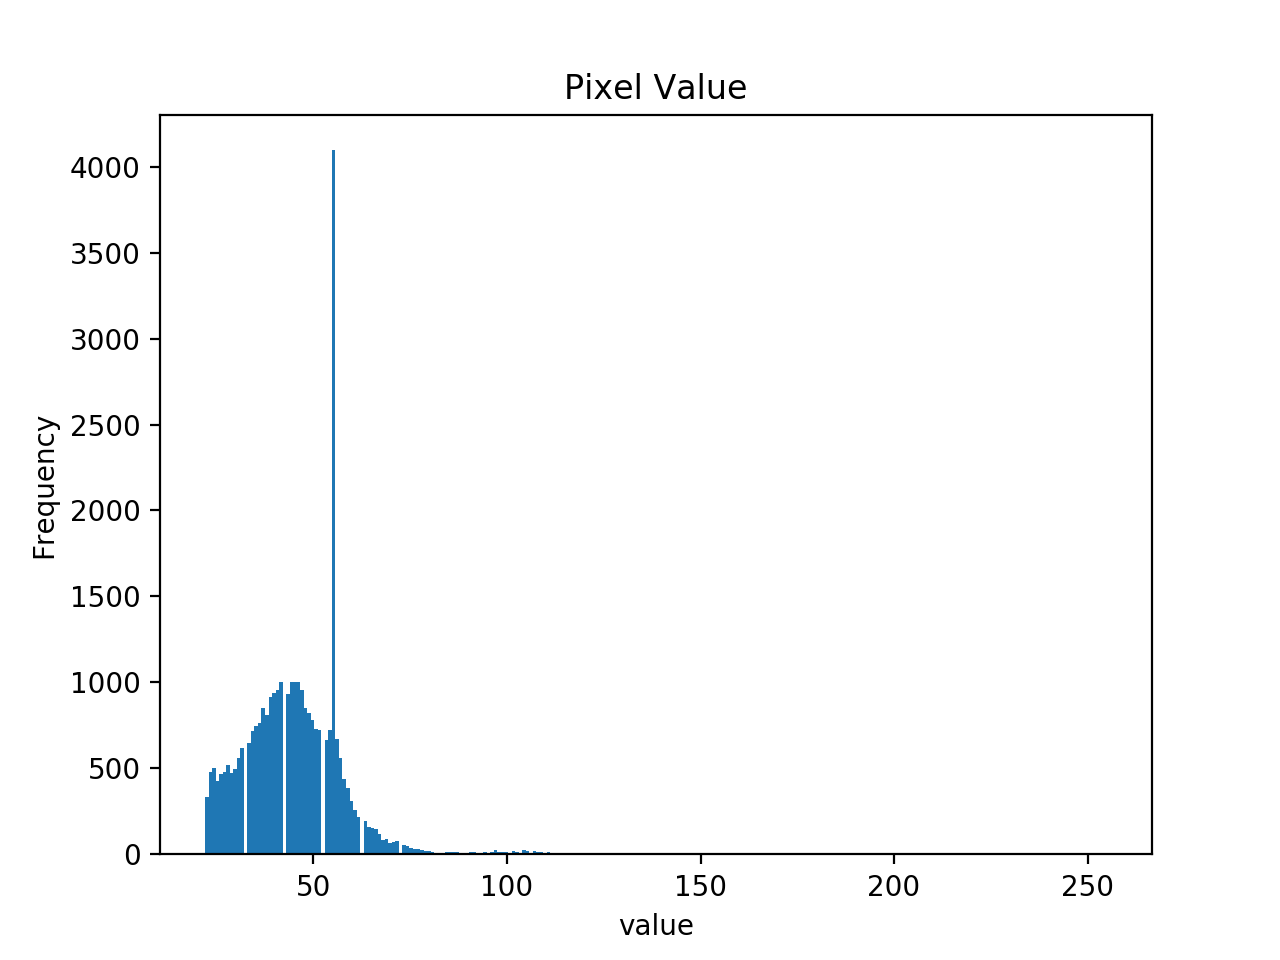
\includegraphics[width=0.7\textwidth]{hist_troublespacing.png}
	\caption{The histogram of the reconstructed image with eliminated values.}
	\label{fig:HistEli}
\end{figure} 

\subsection{Histogram Equalisation}
\label{sec:HistEq}
The histogram equalisation is applied to increase contrast. This is necessary to enhance the structures in the iris. This was implemented manually. As in the noise removal the lowest and highest bin values with more instances than a specified value are found. Based on the values found, the histogram is stretched using the formula in \autoref{eq:hist_stretch}.

\begin{equation}\label{eq:hist_stretch}
	\text{New~Pixel~Value}=(\text{Pixel~Value}-\text{Low~Value})\cdot\frac{255}{\text{High~Value}-\text{Low~Value}}
\end{equation}

The pixels, which have values above $ 255 $ or below $ 0 $ after the formula is applied, are set to $ 255 $ or $ 0 $ respectively. The resulting image is shown in \autoref{fig:irisST}, while \autoref{fig:histST} shows the histogram after applying the formula to each pixel.

\begin{figure}[h]
\centering
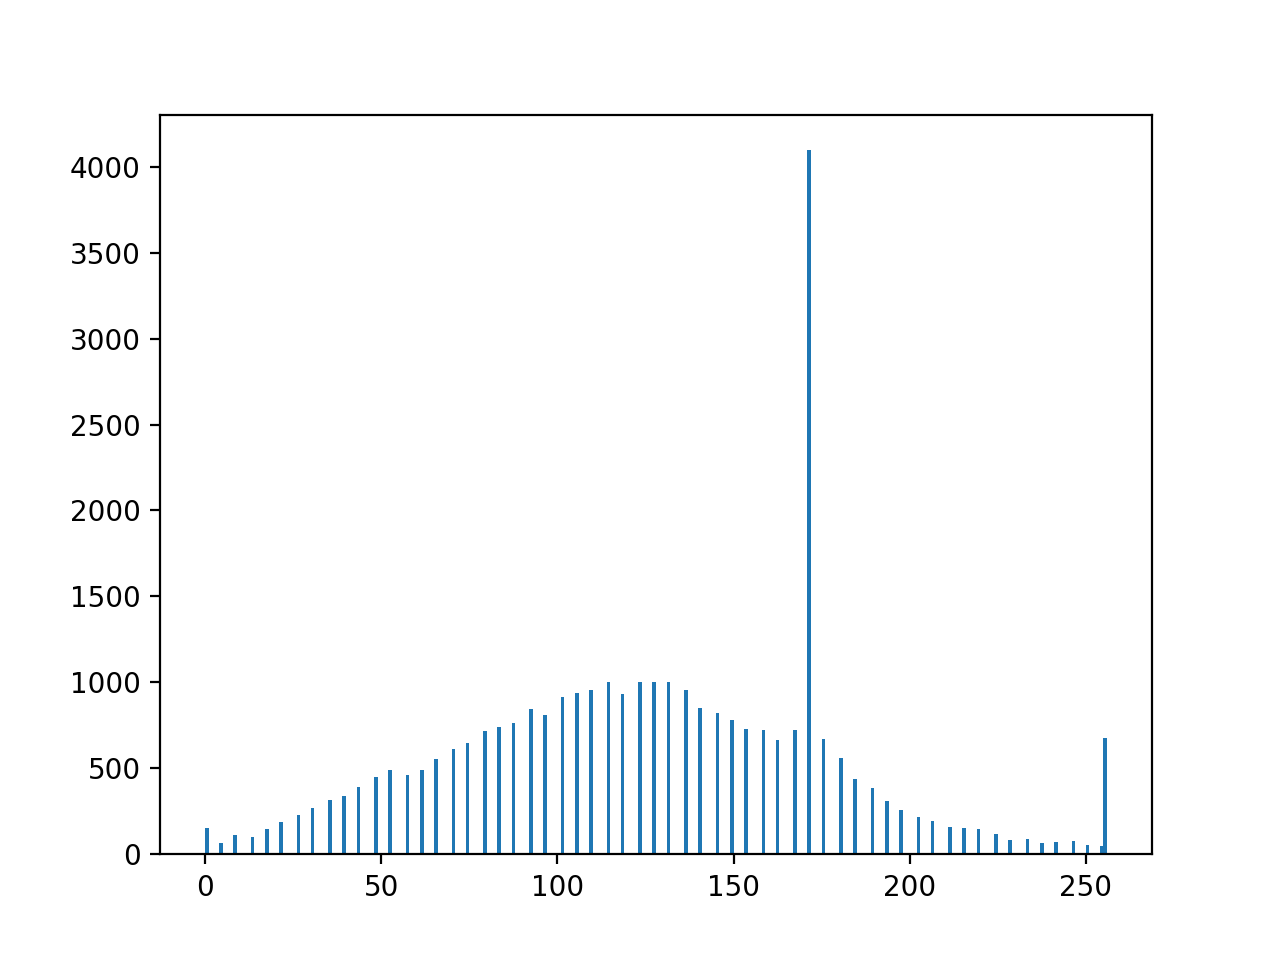
\includegraphics[width=0.7\textwidth]{Stretch_hist.png}
\caption{The histogram of the image after applying the initial "equalise histogram" function.}
\label{fig:histST}
\end{figure}
However, it was discovered that the implemented method was actually histogram stretching, which was mistakenly taken as the same as histogram equalisation. Though the two methods have somewhat the same effects, histogram equalisation is better at ensuring a uniform spreading of the pixels across the histogram. 
This is done by identifying a transform of the bin values which causes the \gls{cdf} of the histogram to be as linear as possible, and apply it to the grey levels or bin values. The result of the histogram equalisation is showed in \autoref{fig:irisEQ} and \autoref{fig:histEQ}.
\begin{figure}[H]
\centering
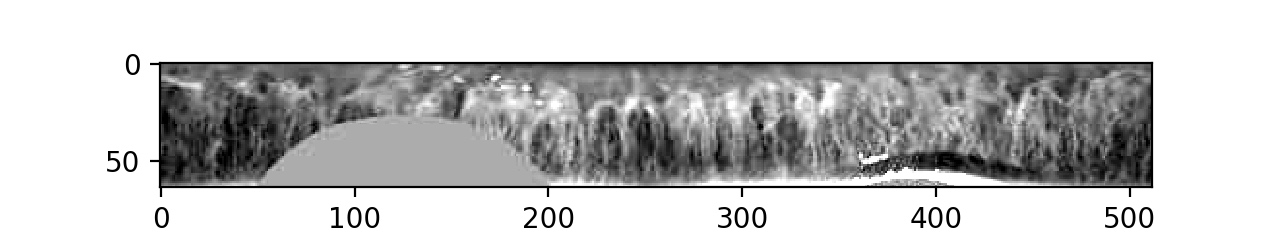
\includegraphics[width=\textwidth]{Stretch_iris.jpg}
\caption{The image of the iris after applying the initial "equalise histogram" function.}
\label{fig:irisST}
\end{figure}
\begin{figure}[H]
\centering
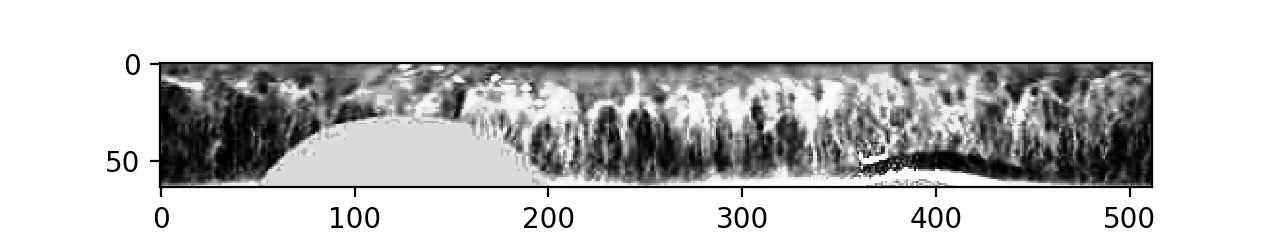
\includegraphics[width=\textwidth]{Equal_iris.jpg}
\caption{The image of the iris after applying the real equalisation of the histogram.}
\label{fig:irisEQ}
\end{figure}
\begin{figure}[h]
\centering
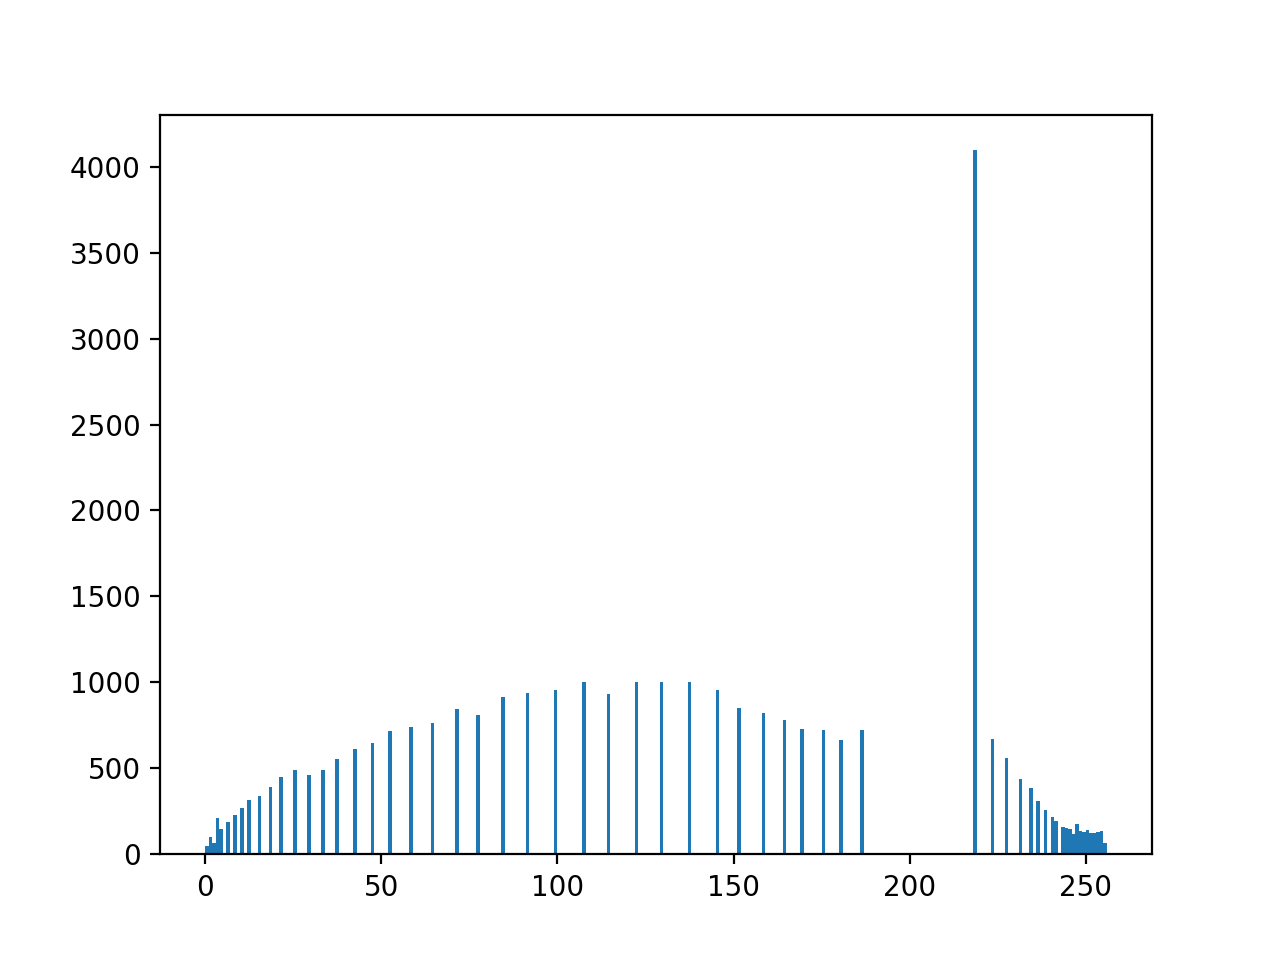
\includegraphics[width=0.7\textwidth]{Equal_hist.png}
\caption{The histogram of the image after applying the real equalisation of the histogram.}
\label{fig:histEQ}
\end{figure}
When comparing the two images of the iris, after applying the two different contrast adjustment methods, it can be concluded that the histogram equalisation does indeed result in better contrast and a more enhanced and out spoken appearance of the structures in the iris than the histogram stretching does. Testing also showed that using the equalisation rather than the stretching increased the accuracy, this is further addressed in \autoref{MachineLearnClassification}. 

\subsection{Feature extraction}
As it is difficult to extract all the complex structures in the iris, the work presented uses the iris image as input. However, because the image in full will result in too large amounts of data to handle during classification, feature extraction is done. Feature vectors are extracted using Haar wavelets in a wavelet decomposition. 
Haar wavelets are a fast and simple way to obtain wavelets. In Haar wavelets, the decomposition is done by calculating the average of neighbouring pixels as well as half the difference between neighbouring pixels. Due to the way the method works the image is lowpass or hi-pass filtered two times in each of the possible combinations. The image of the greatest interest in this case is the one that has been lowpass filtered in both horizontal and vertical direction, this is referred to as LL. This image will be a compressed version of the original image, showing an approximation or the tendency of the original image. The other images created in one stage are HH, HL, LH all of which contain detail coefficients. HH is representing the diagonal detail, while HL presents horizontal detail and LH presents vertical detail. The LL will naturally appear in the upper left corner of the output matrix. 

In order to compress the image sufficiently three stages or passes of Haar wavelet decomposition was carried out. The result is shown in \autoref{fig:haar3}. 
\begin{figure}[h]
\centering
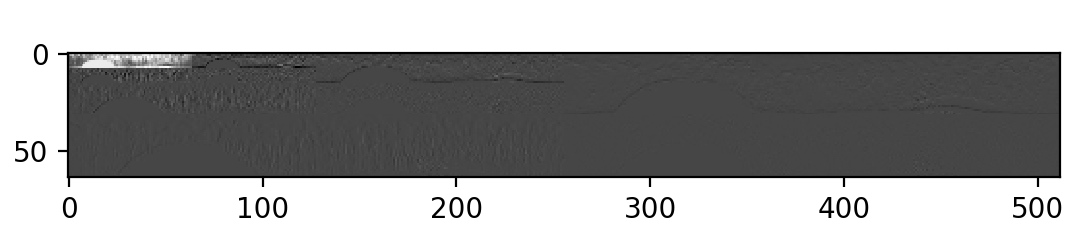
\includegraphics[width=\textwidth]{haar_3.jpg}
\caption{The result of the three level Haar wavelet decomposition. Note that the small light image in the upper left corner is the LL3, which is used onwards.}
\label{fig:haar3}
\end{figure}
The resulting matrix of LL3 coefficients is then put into a feature vector, which is used for training the classifiers described in \autoref{MachineLearnClassification}.

\subsection{Training and Classification}
\label{MachineLearnClassification}
In the work described in the article different classifiers were tested. The best of the investigated classifiers are the \gls{knn}, \gls{lda}, as well as \gls{svm} with linear or quadratic kernel. In the following sections the theory behind the different classifiers is briefly described.

\subsubsection*{K-Nearest Neighbour}
\gls{knn} is one of the most simple supervised classification methods. It is a non-parametric method. This means that the training data is used "raw" and there are no parameters that are deducted from the data in order to form a model. 
 
\gls{knn} utilises Bayes' theorem in order to determine the probability of a sample belonging to a certain class. The probability of the sample belonging to different classes is found by examining the density of datapoints belonging to the different classes among the $k$ nearest neighbours. The probability of a class given the sample can be estimated by the formula in \autoref{eq:classProb}.

 \begin{equation}\label{eq:classProb}
	p(C_k|\text{x})=\frac{K_k}{K}
\end{equation}

Where $C_k$ is a given class, $\text{x}$ is the sample, $K$ is the number of neighbours considered, and $K_k$ is the amount of data points among the $K$ neighbours belonging to the class $C_k$.

Finally, a class is assigned to the sample based on which class has the highest conditional probability.

The value $K$ greatly influences the way the classifier performs. Therefore it is important to determine an optimal value of $K$. This may depend on the performance but also the amount of data that has to be compared with. In this project $K$ is found by determining which value of $K$ for $K\in[1,30]$ results in the best performance. This is done by training on a test set of five images and evaluating the train error. \autoref{fig:misclassK} shows the misclassification error dependent on the value of $K$. As seen in the figure $K=1$ results in the lowest misclassification error, therefore this is used going forth in the project work.  
 \begin{figure}[h]
\centering
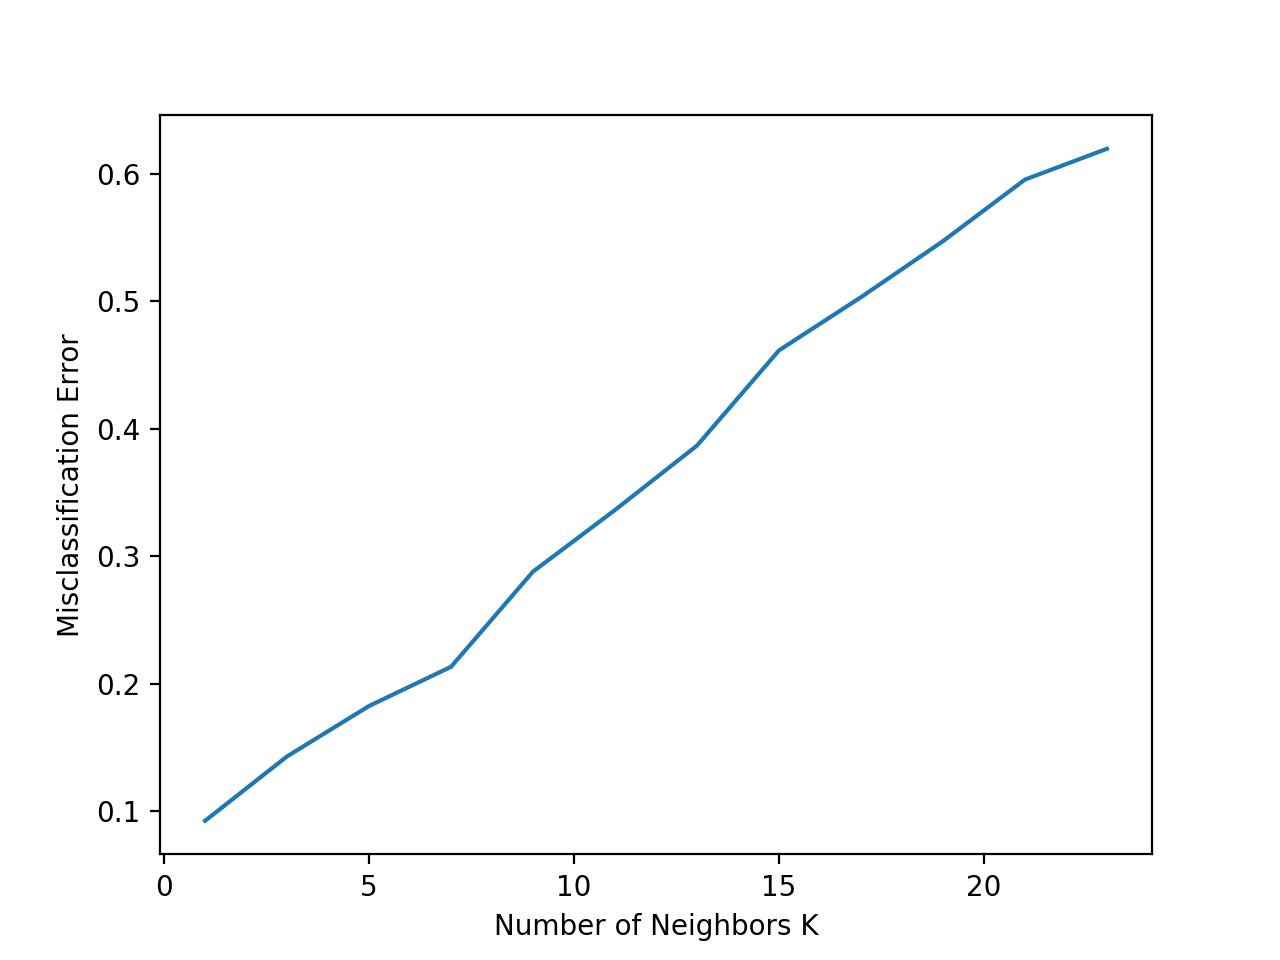
\includegraphics[width=0.8\textwidth]{kgraph.png}
\caption{The misclassification error for the \gls{knn} as a result of the number of neighbours $K$ used for the classifier.}
\label{fig:misclassK}
\end{figure}
\subsubsection*{Linear Discriminant Analysis}
\gls{lda} is a parametric method, which is trained by supervised learning. \gls{lda} is a classifier in which linear decision boundaries are learned based on training data. It is part of a more general group of linear discriminant functions. The decision boundary is found such that interclass variance is maximised while intra class variance is minimised. There are a range of possibilities for identifying the equation for the linear decision border eg. by using SVD or EVD.    

\subsubsection*{Support Vector Machines}
\gls{svm} identifies the optimal linear hyperplane as the decision boundary. The decision borders are found for linearly separable data. A separating hyperplane is not necessarily unique, however, the optimal hyperplane should be unique. The optimal linear decision boundary is found by identifying the hyperplane, which has the maximal margin around it not intersecting with any data points in the training set.
In practice the hyperplane is found based on a subset of data points that lie close to the separating plane, those are called the support vectors.    

However, in some cases the data is not linearly separable. For those cases Kernel Functions can be applied before identifying the optimal hyperplane. The kernel function maps the original data from the original space into a new space, where it can be linearly separated.  

\subsubsection*{Cross Validation}
In this project the above mentioned classification methods are implemented. Just as in the work described in the article cross validation is carried out in order to test the performance of the classifiers. Five images per class are used for the cross validation. The cross validation done is a five fold cross validation. However, since some classes have too few images those classes are neglected. As mentioned in \autoref{sec:HistEq} changing from histogram stretching to histogram equalisation affects the performance of the classifiers. In \autoref{tab:fiveFoldClas} the accuracies as well as the precision of the classifiers in both the case with histogram stretching and histogram equalisation are shown.  

\begin{table}[h]
\centering
\begin{tabular}{|l|c|c|c|c|}
\cline{2-5}
\multicolumn{1}{c|}{}&\multicolumn{2}{c|}{Histogram Stretching}&\multicolumn{2}{c|}{Histogram Equalisation}\\
\hline
Classifier&MA (\%)&$2\sigma$ (\%)&MA (\%)&$2\sigma$ (\%)\\
\hline
KNN (k=1)&$79$&$\pm 6$&$91$&$\pm4$\\
\hline
LDA&$94$&$\pm2$&$95$&$\pm3$\\
\hline
SVM (Linear)&$85$&$\pm8$&$92$&$\pm2$\\
\hline
SVM (quadratic)&$77$&$\pm8$&$92$&$\pm4$\\
\hline
\end{tabular}
\caption{Performance of the different classifiers evaluated by five-fold cross validation. MA is for Mean Accuracy, and $\sigma$ is the standard deviation}
\label{tab:fiveFoldClas}
\end{table} 
Considering the results for the \gls{knn} and the quadratic \gls{svm} shown in \autoref{tab:fiveFoldClas} there seems to be a significant increase in the accuracy of the two classifiers. However, since it is based on such a limited amount of measurements it is probably more representative and valuable to consider the general trends. When comparing the two accuracies across all of the classifiers there seems to be evidence for an increase in accuracy when the histogram equalisation is used rather than the histogram stretching. Therefore the histogram equalisation is used from this point on. 
\begin{table}[h]
\centering
\begin{tabular}{|l|c|c|c|}
\cline{2-4}
\multicolumn{1}{c|}{}&\multicolumn{3}{c|}{Cross Validation Accuracy (\%)}\\
\cline{2-4}
\multicolumn{1}{c|}{}&\cite{Khan2017a}&\multicolumn{2}{c|}{Replicated}\\
\hline
KNN (k=1)&95.1&91&91\\
\hline
LDA&94.28&94&\textbf{95}\\
\hline
SVM (Linear)&96.46&91&92\\
\hline
SVM (quadratic)&\textbf{97}&92&92\\
\hline
\end{tabular}
\caption{Comparison of the performance of the different classifiers achieved by \cite{Khan2017a} and the replicating work in this project. The first column under "Replicated" are accuracies based on data from 55 classes, while the second column is based on data from 91 classes.}
\label{tab:fiveFoldClasCompare}
\end{table} 

In \autoref{tab:fiveFoldClasCompare} the accuracies achieved by the work of \cite{Khan2017a} are compared with the accuracies achieved in the replication of the work when conducting five-fold cross-validation on a set of 5 images from each class. The comparison reveals that the replication does not achieve the same accuracies. In general the original work seems to acquire higher accuracies, however, the original work does not present the variance of the mean accuracy calculated in relation to the cross validation. Therefore, it is impossible to verify how precise the classifiers in the original work are. Another thing to note is the fact that the quadratic \gls{svm} is the one that performs best according to the original work, while the replicated work suggests that the \gls{lda} classifier gives the highest accuracy. There are several factors that might contribute to the difference between the results presented in the original work and the result obtained through replication. One factor might be the amount of data. Though the amount of data samples used per class is the same, the amount of classes is not the same. Due to some issues with processing of the database, which are described in \autoref{sec:ChallDatabase}, only a part of the database was available for testing. First only 55 classes were available and after a while 91 classes of the total 140 classes in the database. Some tests were done with both 55 and 91 classes and the results show that the amount of classes does influence the accuracies as is shown in \autoref{tab:fiveFoldClasCompare}. Another factor that might cause different results is the fact that some steps of the processing are described quite briefly, thus the replication of the work might not be entirely aligned with the original work. 

\begin{table}[h]
\centering
\begin{tabular}{|l|c|c|c|}
\cline{2-4}
\multicolumn{1}{c|}{}&\multicolumn{3}{c|}{Classification accuracy (\%)}\\
\hline
Classifier&Train&Test&Validation\\
\hline
KNN (k=1)&100&96&97\\
\hline
LDA&100&98&97\\
\hline
SVM (Linear)&100&97&98\\
\hline
SVM (quadratic)&100&98&98\\
\hline
\end{tabular}
\caption{The different accuracies achieved by the classifiers when trained on 70\% of the data and tested and validated respectively on 15\% of the data.}
\label{tab:ClasAccMachine}
\end{table} 

In order to examine the performance of the systems implemented in this work when trained on more data a test was conducted. During the test the classifiers were trained on 70\% of the data and were tested on 15\% of the data. Finally they were validated by testing on the remaining 15\% of the data. The results are shown in \autoref{tab:ClasAccMachine}. As the table shows the train accuracies for all the classifiers are 100\%, which means the models are fitted perfectly to the train data. As can be expected, the test and validation accuracies are lower than the train accuracy. It is worth noting that the accuracies are higher than the accuracies obtained in the cross validation based on only a smaller amount of data. Furthermore, the training on more data results in accuracies higher than the ones obtained in cross validation in the original work. However, this test seemingly confirms the statement of the original work that the quadratic \gls{svm} performs best.

Though the achieved accuracies are quite high, the performance of these machine learning methods still cannot compete with the state of the art accuracies within iris classification and general biometric identification methods as described in \autoref{ch:req}. Therefore, another method, deep learning, is investigated for iris classification in order to explore, whether, this method can classify with accuracies comparable to the state of the art performances and comply with the requirement of an accuracy higher than 99\%. The work on the implementation of a \gls{cnn} for iris classification is described in \autoref{sec:cnn_iris_rec}.

\subsection{Challenges}
\label{sec:ChallDatabase}
As mentioned previously several issues were encountered during the implementation of the work described in this chapter. This section elaborates on a few of the issues. 

\subsubsection{Algorithm Description} 
Although overall steps of the processing algorithm are presented in the article by \cite{Khan2017a}, there are a lot of unclear details when considering the descriptions of the individual steps of the processing. This makes it difficult to replicate the work conducted in the article, and it results in parts of the code being implemented based on the best knowledge supplemented with ideas, while other things are based on the indications from tests.

\subsubsection{Processing Issues}
Once the algorithm was implemented it had to be applied in order to process the entire Warsaw-Biobase database consisting of 3192 images of irises obtained from 70 subjects. The handling and processing of this amount of data proved quite troublesome. First of all, the processing of one image using the implemented MATLAB libraries takes quite some time. The time of course depends on the resources of the computer, however, it took a few minutes per image. Furthermore, the process sometimes reported that it was too demanding for the laptops used. Therefore, the processing was moved to be carried out by a desktop PC with more computational power. This was a shared computer borrowed through an internet connection using TeamViewer, which meant that it was only accessible sometimes. 

Another issue was the variation in the images being processed. Though the algorithm is implemented in a way that is somewhat flexible, which automatically identifies the areas of interest, it does sometimes fail. In some cases the algorithm is unable to identify the wanted area or it falsely identifies the wrong area as the area of interest. In those cases the algorithm would break or get stuck, which required manual restart or continuation of the processing. 

The combination of the algorithm not running continuously, and the fact that accessing the running processing was only possible sometimes, made it difficult to ensure that the algorithm was running, and as a result the process would waste large amounts of time being stuck on a single image. Therefore, processing of the full database was not completed, however, 2086 images in 91 classes of the full 140 classes were processed and used for the development and testing in the project work. 










